\begin{frame}{Challenges in Adapting Computation}
  \metroset{block=fill}
  \begin{block}{Goal}
    Adapt computation to different platforms
  \end{block}

  \visible<2->{
    \textbf{Challenges}:

    \begin{enumerate}
    \item Large parameter space
      \visible<3->{
        \begin{itemize}
        \item Previous approaches use random search or coordinate/greedy
          approach
        \item We propose \alert{Bayesian Optimization (BO)} for profiling
        \end{itemize}
      }
    \item Heterogeneous capabilities (and not available when profiling)
      \visible<4->{
        \begin{itemize}
        \item \alert{Profile transfer}: refine existing Pareto-optimal points
        \end{itemize}
      }
    \end{enumerate}
  }
\end{frame}

\begin{frame}{Bayesian Optimization 101}
  Bayesian optimization approximate black-box functions with proxy functions and
  iteratively proposes new sample point in the large parameter space. Effective
  for,

  \pause
  \begin{itemize}
    % https://dhnzl.files.wordpress.com/2016/12/fuzzymad2016_bo_pdf.pdf
    \item Evaluating each sample is expensive.
    \item The objective is a black-box.
    \item The evaluation can be noisy.
  \end{itemize}
  \pause
  \begin{columns}
    \footnotesize
    \column{0.5\textwidth}
    Gaining attraction beyond ML scope:

    \begin{itemize}
    \item CherryPick~\cite{alipourfard2017cherrypick} finds the best cloud
      configurations for big data analytics.
    \item Google optimize chocolate chip cookies
      recipes~\cite{solnik2017bayesian}.
    \end{itemize}

    \pause
    \column{0.5\textwidth}
    \begin{figure}
      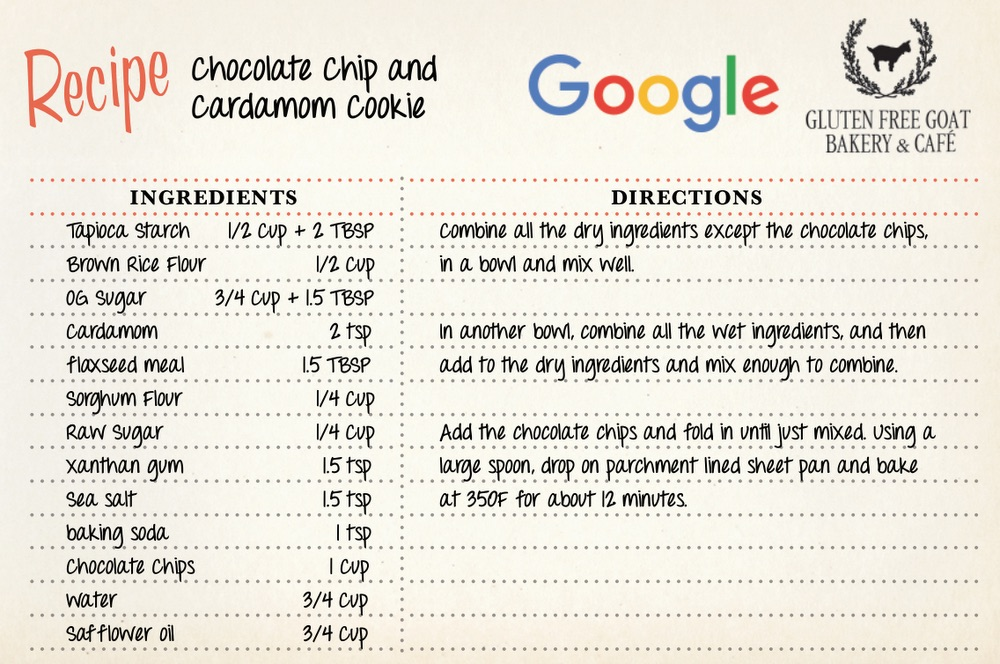
\includegraphics[width=\linewidth]{figures/google-cookie.jpg}
    \end{figure}
  \end{columns}
\end{frame}

\begin{frame}{Bayesian Optimization (Illustrated)}
  \begin{columns}
    \column{0.6\textwidth}
    \begin{figure}
      \centering
      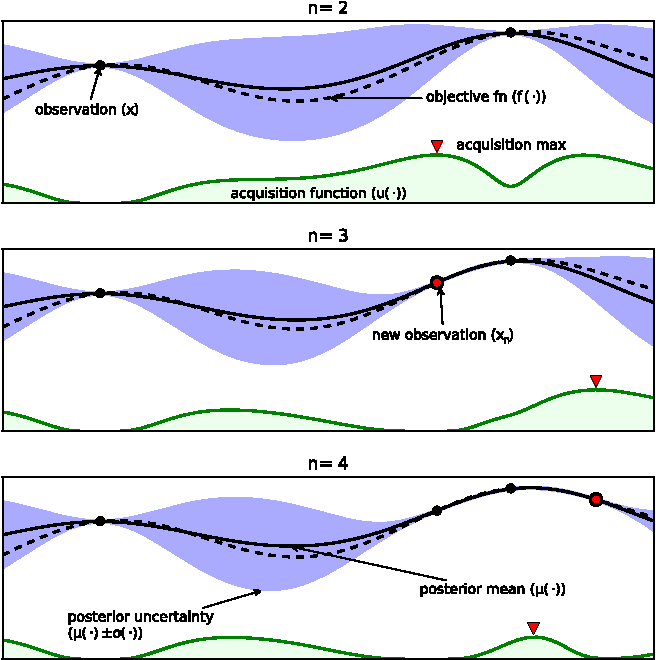
\includegraphics[width=0.8\textwidth]{figures/serving-bo-illustration.pdf}
      \caption{Acquisition function evaluates the utility of candidate points
        for the next evaluation of $f$, balancing a high objective
        (exploitation) and high uncertainty
        (exploration)~\cite{shahriari2016taking}}
    \end{figure}

    \pause
    \column{0.4\textwidth}
    \begin{figure}
      \centering
      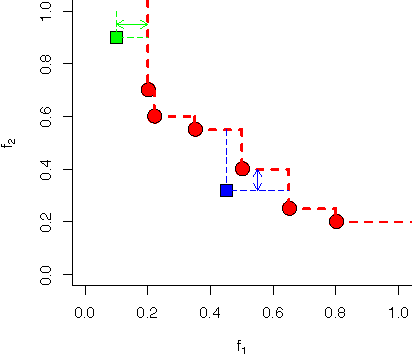
\includegraphics[width=0.8\textwidth]{figures/serving-bo-2d-1.pdf} \\
      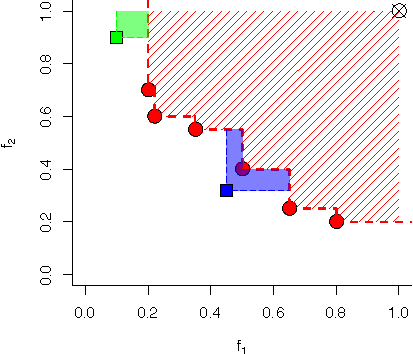
\includegraphics[width=0.8\textwidth]{figures/serving-bo-2d-2.pdf}
      \caption{For two-objective optimization, utility gain is based on
        additive-epsilon (top) or hypervolume (bottom)~\cite{binoisgpareto}}
    \end{figure}
  \end{columns}
\end{frame}

\begin{frame}{Bayesian Optimization For Performance Modeling}
  \vspace{1em} We use PESMO\footnote{A Python package based on
    \href{https://github.com/HIPS/Spearmint}{Spearmint}. It chooses evaluation
    points to maximally reduce the entropy of the posterior distribution over
    the Pareto set.}~\cite{hernandez2016predictive} and compare it with two
  baselines: (1) greedy/coordinate search; (2) random search.

  \pause
  \begin{figure}
    \centering
    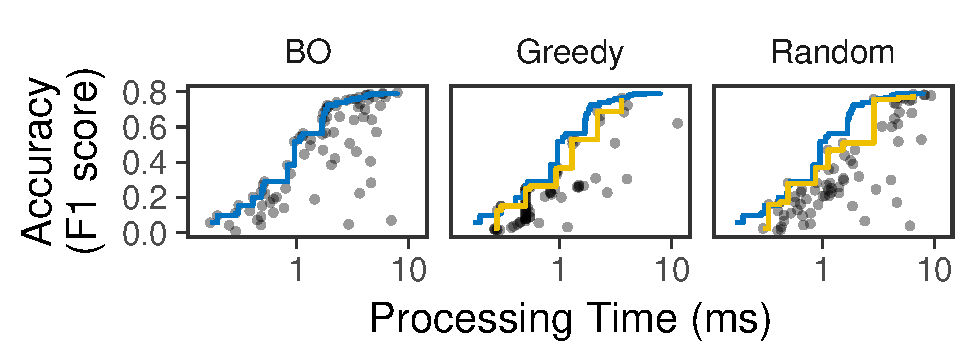
\includegraphics[width=0.95\linewidth]{figures/serving-eval-bo.pdf}
    \caption{BO evaluates 50 configurations and recommends 29 configurations as
      the Pareto-optimal boundary (the blue line). Greedy and Random find
      sub-optimal Pareto configurations with a budget of 80 evaluations (the
      yellow line in each figure).}
  \end{figure}
\end{frame}

\begin{frame}[t]{Profile Transfer (without re-running the entire BO)}
  \vspace{1em}

  We make the following observations:

  \begin{itemize}
    \pause
  \item Accuracy remains for a given algorithm/parameter.
    \pause
  \item Processing time order is preserved
    \begin{itemize}
    \item More expensive algorithms/parameters remain the same across platforms.
    \end{itemize}
    \pause
  \item The ``Pareto-optimal'' is horizontally stretched/compressed.
  \end{itemize}
  \pause
  \begin{figure}
    \centering
    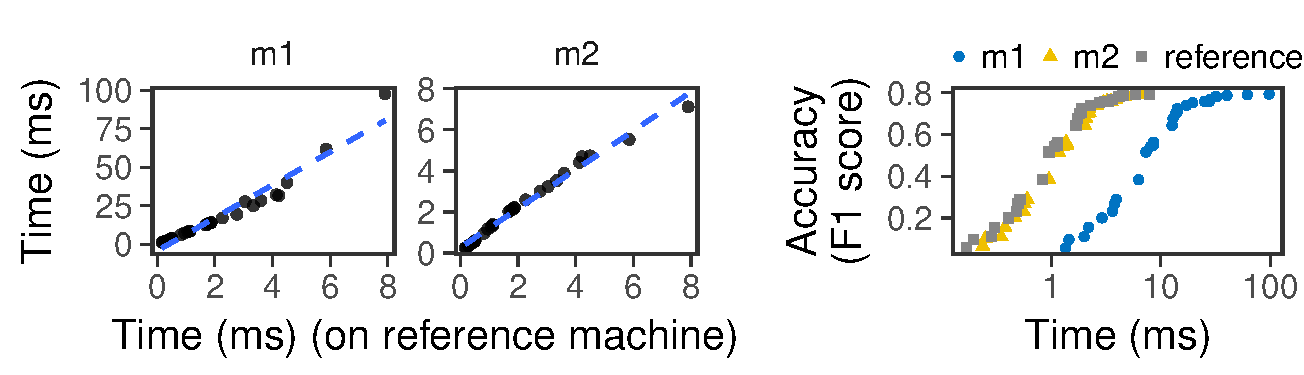
\includegraphics[width=0.95\linewidth]{figures/serving-cross-platform.pdf}
    \caption{(Left) Empirically, processing times follows a linear
      approximation. (Right) Stretched/compressed profile. See paper for
      details.}
  \end{figure}
\end{frame}

%%% Local Variables:
%%% mode: latex
%%% TeX-master: "../talk"
%%% TeX-engine: xetex
%%% End:
